\section{Introduction}
Hydropower is the most mature, reliable and cost-effective
renewable power generation technology available (\cite{brown}), accouting 16
percent of global electricity generation. The global hydropower use and
capacity will increase about 3.1\% each year for the next 25 years (\cite{wi}).
The total investment for large-scale hydropower projects
typically range from USD 1000/kW to around USD 3500/kW and, once commissioned,
the annual operation and maintenance costs of hydropower plants are often
quoted as 4\% of the investment per kW per year (\cite{ecofys}). 

In the specific case of Brazil, the third biggest hydroelectric potential of
the world, hydropower represents 84\% of its electric power total production.
Brazil is the second biggest country of installed hydropower capacity, 84 GW,
and in the Amazon basin, in Madeira river, this number will be increased next
years by the construction of Santo Antonio (3150 MW) and Jirau (3300 MW) power
plants. The dependance on this renewable power source mobilizes private
initiative investments on research centers and universities, and motivates the
development systems with a high degree of automation based on advanced robotics
systems (\cite{aneel}).

A major challenge for hydropower companies is the River water level
control for flooding prevention, dam construction, and maintenance. Several
power plants use the stoplog technology as solution, such as: the Santa Clara
River, in California, USA; the River Great Ouse, in King's Lynn, England; the
Lakefield Generating Station, in Lakefield, Canada; the Killaloe Canal, in
Ireland; and the Goolwa Barrage, in Australia (\ref{figs:intro:goolwa}). 

%in The
%insertion and removal process of stoplogs might have .
\begin{figure}[ht]
\centering
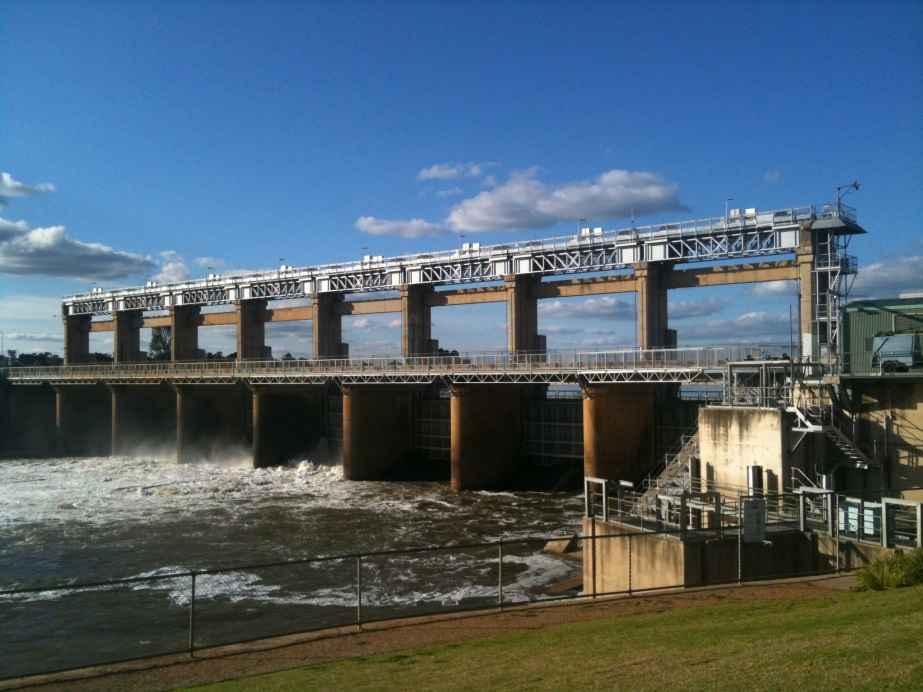
\includegraphics[width=8.4cm]{figs/intro/goolwa.jpg}
\caption{The Goolwa barrage}
\label{figs:intro:goolwa}
\end{figure}

%turbine downtime
%During a routine maintenance, stoplogs, which can close the water flow, are
%installed by lifting beam downstream of turbines.
 
% the resources from remote and hostile environments will increase operation
% costs. Also, the working conditions on offshore installations, characterized
% by unfriendly atmosphere, harsh weather conditions, extreme temperatures,
% constrained space, and the logistical issues are serious obstacles for Oil \&
% Gas companies. In order to be competitive, companies are looking into new and
% better technologies to be able to produce marginal fields and gain new
% resources. The use of robotics in inspection, maintenance, and repair
% operations in Oil \& Gas facilities could greatly improve efficiency, health
% and safety, while decreasing operational and logistics costs.
% It is highly expensive to have people working on the rig, as they
% must be housed and protected, there are costs with personal benefits such as
% health care, and the companies need to evacuate personnel quickly
% in case of an emergency.
% for cost reduction motivates

Recent studies forecast a substantial decrease in the level of human operation
and an increase in automation on future oil fields .
The studies also point out the potential increase
in efficiency and productivity with robot operators, besides of the improvement in
Health, Safety, and Environment (HSE) conditions, as robots can replace humans
in tasks performed in unhealthy, hazardous, and confined areas.
lists the challenges of robotics and automation in Oil
\& Gas industry:%and lists the most important requirements for robotic systems:

\begin{enumerate}[i)]
\item The \emph{atmospheric conditions} on offshore platforms are quite unfriendly, as
hydrocarbon resources can generate explosive and toxic gases;\\ %The robot should be certified to operate in explosive environments.
\item \emph{Corrosive agents}: splashy salty water, salty air and corrosive chemicals;\\
\item \emph{Weather}: high speed wind, squalls, rain and hail. The relative humidity is up to
100\% and ambient temperature can vary between $-30^{\circ}$C to $50^{\circ}$C. Possibly highly radiant heat from equipment and direct sunlight;\\
\item \emph{Constrained space} and/or walkways. Complex structures such as pipes,
flanges, tanks, and stairways.
\end{enumerate}

%There are different kinds of robots in the oil \& gas industry such as
%underwater pipeline repair robotic systems, robots for inspection of valve and
%lever position, gas level or leakage and acoustic anomalies monitoring, and
%robots for identify and locate fire.

Currently, the majority of the robotic systems in the Oil \& Gas industry are
used for subsea tasks, such as mapping of the seabed, and inspection operation
and repair of underwater equipment, risers and pipelines. However, recent
research has focused on robotic applications on the topside of platforms to
perform inspection and maintenance tasks, which includes valve and lever
manipulation, gas level and leakage monitoring, acoustic anomalies diagnosis,
and identification of smoke and fire.
%Guilherme: Senti falta de refs para a parte do subsea

The MIMROex inspection robot  was developed and
tested by the Fraunhofer Institute of Manufacturing Engineering and Automation
(IPA). The robot is capable o.f safely navigate in offshore environments, and
autonomously execute inspection tasks. Sensabot , a
teleoperated inspection robot developed by Carnegie Mellon University, was
designed for severe weather and atmosphere, being certified to operate in toxic, flammable and explosive environments. The SINTEF Topside Robotic System, developed in the robotic lab facility in
Trondheim, Norway, is an intelligent instrumentation system designed to enable onshore operators
to monitor and control the platform's processes .


%The robot includes the following sensors:
%\begin{enumerate}[i)]
%    \item Hydrocarbon sensor
%    \item Pan/tilt/zoom camera for remote operations
%    \item Temperature sensors
%    \item Vibration sensor for pumps, motors and bearings inspection
%    \item Microphone to detect audible machinery problems
%    \item Video camera to detect obstacles
%\end{enumerate}

 
%In this paper, we describe the DORIS project, which aims to develop a mobile
%robot to perform monitoring and inspection in an
%offshore platform. To this end, the system must be able to move throughout the
%monitored environment carrying different sensors, analyzing sensor data
%\emph{in loco} or storing it for a posterior analysis, and interpreting the
%results. The sensors can identify abnormalities such as intruders in restricted
%areas, abandoned objects, smoke, fire, and liquid and gas leakages.
%Furthermore, the robot is able to make machinery diagnosis, read instruments,
%and takes samples using an embedded manipulator (\cite{cba}).

In this paper, we present a general overview of the DORIS robot, and a detailed description of the embedded electronics, power supply system and software architecture. The robot is designed to perform monitoring and inspection tasks in an
offshore platform, being able to move throughout the monitored environment carrying different sensors, analyzing sensor data \emph{in loco} or storing it for a posterior analysis, and interpreting the results. The sensors can identify abnormalities such as intruders in restricted areas, abandoned objects, smoke, fire, and liquid and gas leakages.
The robot is able to make machinery diagnosis, read instruments, and takes samples using an embedded manipulator (\cite{cba}).

This text is organized as follows: a general overview of the robot and its main
challenges are presented in Section \ref{sec:general_overview}, detailed
descriptions of the embedded electronics, the vehicle support system, power
supply system, and software architecture are taken in
Sections \ref{sec:electronics_overview}, \ref{sec:powersupply_overview}, and
\ref{sec:software} respectively.
In Section \ref{sec:results}, preliminary results are shown, and concluding
remarks are drawn in Section \ref{sec:conclusions}.